\documentclass[10pt]{beamer} % aspect ratio 4:3, 128 mm by 96 mm
%\documentclass[10pt,aspectratio=169]{beamer} % aspect ratio 16:9
\graphicspath{{../journal_papers/Elsevier/figs/}}
%\includeonlyframes{frame1,frame2,frame3}
%%%%%%%%%%%%%%%%%%%%%%%%%%%%%%%%%%%%%%%%%%%%%%%%%%
% Packages
%%%%%%%%%%%%%%%%%%%%%%%%%%%%%%%%%%%%%%%%%%%%%%%%%%
\usepackage{appendixnumberbeamer}
\usepackage{booktabs}
\usepackage[scale=2]{ccicons}
\usepackage{pgfplots}
\usepackage{xspace}
\usepackage{amsmath}
\usepackage{totcount}
\usepackage{tikz}
%\usepackage{comment}
%\usetikzlibrary{external} % speedup compilation
%\tikzexternalize % activate!
%\usetikzlibrary{shapes,arrows}  

%\usepackage{bibentry}

\usepackage{caption}%
\captionsetup[figure]{labelformat=empty}%
%%%%%%%%%%%%%%%%%%%%%%%%%%%%%%%%%%%%%%%%%%%%%%%%%%
% Metropolis theme custom modification file
%%%%%%%%%%%%%%%%%%%%%%%%%%%%%%%%%%%%%%%%%%%%%%%%%%
% Metropolis theme custom modification file
%%%%%%%%%%%%%%%%%%%%%%%%%%%%%%%%%%%%%%%%%%%%%%%%%%
% Metropolis theme custom colors
%%%%%%%%%%%%%%%%%%%%%%%%%%%%%%%%%%%%%%%%%%%%%%%%%%
\usetheme[progressbar=foot]{metropolis}
\useoutertheme{metropolis}
\useinnertheme{metropolis}
\usefonttheme{metropolis}
\setbeamercolor{background canvas}{bg=white}

%\usecolortheme{spruce}

\definecolor{myblue}{rgb}{0.19,0.55,0.91}
\definecolor{mediumblue}{rgb}{0,0,205}
\definecolor{darkblue}{rgb}{0,0,139}
\definecolor{Dodgerblue}{HTML}{1E90FF}
\definecolor{Navy}{HTML}{000080} % {rgb}{0,0,128}
\definecolor{Aliceblue}{HTML}{F0F8FF}
\definecolor{Lightskyblue}{HTML}{87CEFA}
\definecolor{logoblue}{RGB}{1,67,140}
\definecolor{Purple}{HTML}{911146}
\definecolor{Orange}{HTML}{CF4A30}

\setbeamercolor{progress bar}{bg=Lightskyblue}
\setbeamercolor{progress bar}{ fg=logoblue} 
\setbeamercolor{frametitle}{bg=logoblue}
\setbeamercolor{title separator}{fg=logoblue}
\setbeamercolor{block title}{bg=Lightskyblue!30,fg=black}
\setbeamercolor{block body}{bg=Lightskyblue!15,fg=black}
\setbeamercolor{alerted text}{fg=Purple}
%%%%%%%%%%%%%%%%%%%%%%%%%%%%%%%%%%%%%%%%%%%%%%%%%%
%  Theme modifications
%%%%%%%%%%%%%%%%%%%%%%%%%%%%%%%%%%%%%%%%%%%%%%%%%%
% modify progress bar linewidth
\makeatletter
\setlength{\metropolis@progressinheadfoot@linewidth}{2pt} 
\setlength{\metropolis@titleseparator@linewidth}{1pt}
\setlength{\metropolis@progressonsectionpage@linewidth}{1pt}

\setbeamertemplate{progress bar in section page}{
	\setlength{\metropolis@progressonsectionpage}{%
		\textwidth * \ratio{\thesection pt}{\totvalue{totalsection} pt}%
	}%
	\begin{tikzpicture}
	\fill[bg] (0,0) rectangle (\textwidth, \metropolis@progressonsectionpage@linewidth);
	\fill[fg] (0,0) rectangle (\metropolis@progressonsectionpage, \metropolis@progressonsectionpage@linewidth);
	\end{tikzpicture}%
}
\makeatother
\newcounter{totalsection}
\regtotcounter{totalsection}

\AtBeginDocument{%
	\pretocmd{\section}{\refstepcounter{totalsection}}{\typeout{Yes, prepending was successful}}{\typeout{No, prepending was not successful}}%
}%
%%%%%%%%%%%%%%%%%%%%%%%%%%%%%%%%%%%%%%%%%%%%%%%%%%
%  Bibliography mods
%%%%%%%%%%%%%%%%%%%%%%%%%%%%%%%%%%%%%%%%%%%%%%%%%%
\setbeamertemplate{bibliography item}{\insertbiblabel} %% Remove book symbol from references and add number in square brackets
% kill the abominable icon (without number)
%\setbeamertemplate{bibliography item}{}
%\makeatletter
%\renewcommand\@biblabel[1]{#1.} % number only
%\makeatother
% remove line breaks in bibliography
\setbeamertemplate{bibliography entry title}{}
\setbeamertemplate{bibliography entry location}{}
%%%%%%%%%%%%%%%%%%%%%%%%%%%%%%%%%%%%%%%%%%%%%%%%%%
%  Bibliography custom commands
%%%%%%%%%%%%%%%%%%%%%%%%%%%%%%%%%%%%%%%%%%%%%%%%%%
\newcommand{\bibliotitlestyle}[1]{\textbf{#1}\par}

\newif\ifinbiblio
\newcounter{bibkey}
\newenvironment{biblio}[2][long]{%
    %\setbeamertemplate{bibliography item}{\insertbiblabel}
    \setbeamertemplate{bibliography item}{}% without numbers
	\setbeamerfont{bibliography item}{size=\footnotesize}
	\setbeamerfont{bibliography entry author}{size=\footnotesize}
	\setbeamerfont{bibliography entry title}{size=\footnotesize}
	\setbeamerfont{bibliography entry location}{size=\footnotesize}
	\setbeamerfont{bibliography entry note}{size=\footnotesize}
	\ifx!#2!\else%
	\bibliotitlestyle{#2}%
	\fi%
	\begin{thebibliography}{}%
		\inbibliotrue%
		\setbeamertemplate{bibliography entry title}[#1]%
	}{%
		\inbibliofalse%
		\setbeamertemplate{bibliography item}{}%
	\end{thebibliography}%
}

\newcommand{\biblioref}[5][short]{
	\setbeamertemplate{bibliography entry title}[#1]
	\stepcounter{bibkey}%
	\ifinbiblio%
	\bibitem{\thebibkey}%
	#2
	\newblock #4
	\ifx!#5!\else\newblock {\em #5}, #3 \fi%
	\else%
	\begin{biblio}{}
		\bibitem{\thebibkey}
		#2
		\newblock #4
		\ifx!#5!\else\newblock {\em #5}, #3\fi
	\end{biblio}
	\fi
}
%
%\newbibmacro*{hypercite}{%
%	\renewcommand{\@makefntext}[1]{\noindent\normalfont##1}%
%	\footnotetext{%
%		\blxmkbibnote{foot}{%
%			\printtext[labelnumberwidth]{%
%				\printfield{prefixnumber}%
%				\printfield{labelnumber}}%
%			\addspace
%			\fullcite{\thefield{entrykey}}}}}
%
%\DeclareCiteCommand{\hypercite}%
%{\usebibmacro{cite:init}}
%{\usebibmacro{hypercite}}
%{}
%{\usebibmacro{cite:dump}}
%
%% Redefine the \footfullcite command to use the reference number
%\renewcommand{\footfullcite}[1]{\cite{#1}\hypercite{#1}}
%%%%%%%%%%%%%%%%%%%%%%%%%%%%%%%%%%%%%%%%%%%%%%%%%%
% Custom commands
%%%%%%%%%%%%%%%%%%%%%%%%%%%%%%%%%%%%%%%%%%%%%%%%%%
% matrix command 
\newcommand{\matr}[1]{\mathbf{#1}} % bold upright (Elsevier, Springer)
%\newcommand{\matr}[1]{#1}          % pure math version
%\newcommand{\matr}[1]{\bm{#1}}     % ISO complying version
% vector command 
\newcommand{\vect}[1]{\mathbf{#1}} % bold upright (Elsevier, Springer)
\newcommand{\ud}{\mathrm{d}}
\renewcommand{\vec}[1]{\mathbf{#1}}
\newcommand{\veca}[2]{\mathbf{#1}{#2}}
\newcommand{\bm}[1]{\mathbf{#1}}
\newcommand{\bs}[1]{\boldsymbol{#1}}
% derivative upright command
\DeclareRobustCommand*{\drv}{\mathop{}\!\mathrm{d}}
% 
\newcommand{\themename}{\textbf{\textsc{metropolis}}\xspace}

%%%%%%%%%%%%%%%%%%%%%%%%%%%%%%%%%%%%%%%%%%%%%%%%%%
%  Title page options
%%%%%%%%%%%%%%%%%%%%%%%%%%%%%%%%%%%%%%%%%%%%%%%%%%
% \date{\today}
\date{15.08.2019}
%%%%%%%%%%%%%%%%%%%%%%%%%%%%%%%%%%%%%%%%%%%%%%%%%%
% option 1
%%%%%%%%%%%%%%%%%%%%%%%%%%%%%%%%%%%%%%%%%%%%%%%%%%
%\title{Parallel spectral element method for guided wave based structural health monitoring}
%\subtitle{}
%\author{\textbf{Paweł Kudela}\\Jochen Moll \\Piotr Fiborek}
% logo align to Institute 
%\institute{Institute of Fluid Flow Machinery\\Polish Academy of Sciences \\ \vspace{-1.5cm}\flushright \includegraphics[width=4cm]{../images/logo/logo_eng_40mm.eps}}
%\institute{Institute of Fluid Flow Machinery\\Polish Academy of Sciences \\ \vspace{-1.5cm}}
%%%%%%%%%%%%%%%%%%%%%%%%%%%%%%%%%%%%%%%%%%%%%%%%%%
% option 2 - authors in one line
%%%%%%%%%%%%%%%%%%%%%%%%%%%%%%%%%%%%%%%%%%%%%%%%%%
	\title{Parallel spectral element method for guided wave based structural health monitoring}
%	\subtitle{Lamb-opt}
	\author{\textbf{Paweł Kudela}\textsuperscript{1}, Jochen Moll\textsuperscript{2}, Piotr Fiborek\textsuperscript{1} }
%	% logo align to Institute 
%	\institute{\textsuperscript{1}Xi'an Jiaotong University \\ \textsuperscript{2}Institute of Fluid Flow Machinery\\ \hspace*{1pt} Polish Academy of Sciences \\ \vspace{-1.5cm}\flushright \includegraphics[width=4cm]{../images/logo/logo_eng_40mm.eps}}
	\institute{ \textsuperscript{1}Institute of Fluid Flow Machinery\\ \hspace*{1pt} Polish Academy of Sciences \\ \\ \textsuperscript{2}J.W. Goethe University\\ \hspace*{1pt} Department of Physics \vspace{-1.5cm}}
%%%%%%%%%%%%%%%%%%%%%%%%%%%%%%%%%%%%%%%%%%%%%%%%%%
% option 3 - multilogo vertical
%%%%%%%%%%%%%%%%%%%%%%%%%%%%%%%%%%%%%%%%%%%%%%%%%%
%\title{Elastic constants identification of composite laminates by using Lamb wave dispersion curves and optimization methods}
%\subtitle{Lamb-opt}
%	\author{\textbf{Paweł Kudela}\inst{1}, Maciej Radzieński\inst{1}, Wiesław Ostachowicz\inst{1}, Zhibo Yang\inst{2} }
%	% logo under Institute 
%	\institute%
%	{ 
%		\inst{1}%
%		Institute of Fluid Flow Machinery\\ \hspace*{1pt} Polish Academy of Sciences \\ \includegraphics[height=0.85cm]{../images/logo/logo_eng_40mm.eps} \\
%		\and
%		\inst{2}%
%	    Xi'an Jiaotong University \\ \includegraphics[height=0.85cm]{../images/logo/logo_box.eps}
%    }
% end od option 3
%%%%%%%%%%%%%%%%%%%%%%%%%%%%%%%%%%%%%%%%%%%%%%%%%%
%% option 4 - 3 Institutes and logos horizontal centered
%%%%%%%%%%%%%%%%%%%%%%%%%%%%%%%%%%%%%%%%%%%%%%%%%%
%\title{Elastic constants identification of composite laminates by using Lamb wave dispersion curves and optimization methods}
%\subtitle{Lamb-opt }
%\author{\textbf{Paweł Kudela}\textsuperscript{1}, Maciej Radzieński\textsuperscript{1}, Marco Miniaci\textsuperscript{2}, Zhibo Yang\textsuperscript{3} }
%
%\institute{ 
%\begin{columns}[T,onlytextwidth]
%	\column{0.39\textwidth}
%	\begin{center}
%		\textsuperscript{1}Institute of Fluid Flow Machinery\\ \hspace*{3pt}Polish Academy of Sciences
%	\end{center}
%	\column{0.3\textwidth}
%	\begin{center}
%		\textsuperscript{2}Zurich University
%	\end{center}
%	\column{0.3\textwidth}
%	\begin{center}
%		\textsuperscript{3}Xi'an Jiaotong University
%	\end{center}
%\end{columns}
%\vspace{6pt}
%% logos 
%\begin{columns}[b,onlytextwidth]
%	\column{0.39\textwidth}
%		\centering 
%		\includegraphics[width=\textwidth,height=0.85cm,keepaspectratio]{../images/logo/logo_eng_40mm.eps}
%	\column{0.3\textwidth}
%		\centering 
%		\includegraphics[width=\textwidth,height=0.85cm,keepaspectratio]{../images/logo/logo_box.eps}
%	\column{0.3\textwidth}
%		\centering 
%		\includegraphics[width=\textwidth,height=0.85cm,keepaspectratio]{../images/logo/logo_box2.eps}
%\end{columns}
%}
%\makeatletter
%\setbeamertemplate{title page}{
%	\begin{minipage}[b][\paperheight]{\textwidth}
%		\centering  % <-- Center here
%		\ifx\inserttitlegraphic\@empty\else\usebeamertemplate*{title graphic}\fi
%		\vfill%
%		\ifx\inserttitle\@empty\else\usebeamertemplate*{title}\fi
%		\ifx\insertsubtitle\@empty\else\usebeamertemplate*{subtitle}\fi
%		\usebeamertemplate*{title separator}
%		\ifx\beamer@shortauthor\@empty\else\usebeamertemplate*{author}\fi
%		\ifx\insertdate\@empty\else\usebeamertemplate*{date}\fi
%		\ifx\insertinstitute\@empty\else\usebeamertemplate*{institute}\fi
%		\vfill
%		\vspace*{1mm}
%	\end{minipage}
%}
%
%\setbeamertemplate{title}{
%	%  \raggedright%  % <-- Comment here
%	\linespread{1.0}%
%	\inserttitle%
%	\par%
%	\vspace*{0.5em}
%}
%\setbeamertemplate{subtitle}{
%	%  \raggedright%  % <-- Comment here
%	\insertsubtitle%
%	\par%
%	\vspace*{0.5em}
%}
%\makeatother
% end of option 4
%%%%%%%%%%%%%%%%%%%%%%%%%%%%%%%%%%%%%%%%%%%%%%%%%%
% option 5 - 2 Institutes and logos horizontal centered
%%%%%%%%%%%%%%%%%%%%%%%%%%%%%%%%%%%%%%%%%%%%%%%%%%
%\title{Elastic constants identification of composite laminates by using Lamb wave dispersion curves and optimization methods}
%\subtitle{Lamb-opt }
%\author{\textbf{Paweł Kudela}\textsuperscript{1}, Maciej Radzieński\textsuperscript{1}, Marco Miniaci\textsuperscript{2}}
%
%\institute{ 
%	\begin{columns}[T,onlytextwidth]
%		\column{0.5\textwidth}
%			\centering
%			\textsuperscript{1}Institute of Fluid Flow Machinery\\ \hspace*{3pt}Polish Academy of Sciences
%		\column{0.5\textwidth}
%			\centering
%			\textsuperscript{2}Zurich University
%	\end{columns}
%	\vspace{6pt}
%	% logos 
%	\begin{columns}[b,onlytextwidth]
%		\column{0.5\textwidth}
%		\centering 
%		\includegraphics[width=\textwidth,height=0.85cm,keepaspectratio]{../images/logo/logo_eng_40mm.eps}
%		\column{0.5\textwidth}
%		\centering 
%		\includegraphics[width=\textwidth,height=0.85cm,keepaspectratio]{../images/logo/logo_box.eps}
%	\end{columns}
%}
%\makeatletter
%\setbeamertemplate{title page}{
%	\begin{minipage}[b][\paperheight]{\textwidth}
%		\centering  % <-- Center here
%		\ifx\inserttitlegraphic\@empty\else\usebeamertemplate*{title graphic}\fi
%		\vfill%
%		\ifx\inserttitle\@empty\else\usebeamertemplate*{title}\fi
%		\ifx\insertsubtitle\@empty\else\usebeamertemplate*{subtitle}\fi
%		\usebeamertemplate*{title separator}
%		\ifx\beamer@shortauthor\@empty\else\usebeamertemplate*{author}\fi
%		\ifx\insertdate\@empty\else\usebeamertemplate*{date}\fi
%		\ifx\insertinstitute\@empty\else\usebeamertemplate*{institute}\fi
%		\vfill
%		\vspace*{1mm}
%	\end{minipage}
%}
%
%\setbeamertemplate{title}{
%	%  \raggedright%  % <-- Comment here
%	\linespread{1.0}%
%	\inserttitle%
%	\par%
%	\vspace*{0.5em}
%}
%\setbeamertemplate{subtitle}{
%	%  \raggedright%  % <-- Comment here
%	\insertsubtitle%
%	\par%
%	\vspace*{0.5em}
%}
%\makeatother
% end of option 5
%
%%%%%%%%%%%%%%%%%%%%%%%%%%%%%%%%%%%%%%%%%%%%%%%%%%
%  End of title page options
%%%%%%%%%%%%%%%%%%%%%%%%%%%%%%%%%%%%%%%%%%%%%%%%%%
% logo option - alternative manual insertion by modification of coordinates in \put()
%\titlegraphic{%
%	%\vspace{\logoadheight}
%	\begin{picture}(0,0)
%	\put(305,-185){\makebox(0,0)[rb]{\includegraphics[width=4cm]{../images/logo/logo_eng_40mm.eps}}}
%	\end{picture}}
%
%%%%%%%%%%%%%%%%%%%%%%%%%%%%%%%%%%%%%%%%%%%%%%%%%%
%\tikzexternalize % activate!
%%%%%%%%%%%%%%%%%%%%%%%%%%%%%%%%%%%%%%%%%%%%%%%%%%
\begin{document}
%%%%%%%%%%%%%%%%%%%%%%%%%%%%%%%%%%%%%%%%%%%%%%%%%%
\maketitle
%%%%%%%%%%%%%%%%%%%%%%%%%%%%%%%%%%%%%%%%%%%%%%%%%%
% SLIDES
%%%%%%%%%%%%%%%%%%%%%%%%%%%%%%%%%%%%%%%%%%%%%%%%%%
\begin{frame}{Table of contents}
  \setbeamertemplate{section in toc}[sections numbered]
  \tableofcontents[hideallsubsections]
\end{frame}
%%%%%%%%%%%%%%%%%%%%%%%%%%%%%%%%%%%%%%%%%%%%%%%%%%
\section{Introduction}
%%%%%%%%%%%%%%%%%%%%%%%%%%%%%%%%%%%%%%%%%%%%%%%%%%
\begin{frame}[fragile,label=frame1]{Funding}
	
	NAWA – Polish National Agency for Academic Exchange
	
	Mobility project to carry out research at Johann Wolfgang Goethe University, Frankfurt am Main, Germany, 2019 (3 months)
	
	\emph{Towards model assisted structural health monitoring}
	
\end{frame}
%%%%%%%%%%%%%%%%%%%%%%%%%%%%%%%%%%%%%%%%%%%%%%%%%%
\begin{frame}[fragile,label=frame2]{Context}
	
	National Science Centre, Poland
	
	2019--2021 (3 years)
	
  	\emph{Feasibility studies of artificial intelligence-driven diagnostics}
  
\end{frame}
%%%%%%%%%%%%%%%%%%%%%%%%%%%%%%%%%%%%%%%%%%%%%%%%%%
\begin{frame}[label=frame3]{Small project within big project}
	\begin{figure}
		\centering
		\only<1>{
		\includegraphics[width=\textwidth]{beamer_figs/Plan-scheme-nn-small-eng.png}	
		\label{fig:plan_scheme}
		}
		\only<2>{
		\includegraphics[width=\textwidth]{beamer_figs/Plan-scheme-nn-small-eng2.png}	
		\label{fig:plan_scheme2}
		}
	\end{figure}	
\end{frame}
%%%%%%%%%%%%%%%%%%%%%%%%%%%%%%%%%%%%%%%%%%%%%%%%%%
\begin{frame}[t]{Motivation}
	\biblioref{C.A.C Leckey, K.R. Wheeler,V.N. Hafiychuk, H. Hafiychuk, D.A. Timucin}{2018}{Simulation of guided-wave ultrasound propagation in composite laminates: Benchmark comparisons of numerical codes and experiment}{Ultrasonics}
	\begin{figure}
		\includegraphics[width=\textwidth]{beamer_figs/Leckey-2018-table.png}
		\caption{Performance metrics of commercial software for wave propagation modelling}
	\label{fig:Leckey_table}
	\end{figure}
	\begin{alertblock}{Potential Problems}
		Shortest run time \textbf{19.5 h} is for COMSOL but requires huge amount of~memory space\\
		19.5 h $\times$ 1000 simulations $\approx$ \textbf{812 days}
	\end{alertblock}
\end{frame}
%%%%%%%%%%%%%%%%%%%%%%%%%%%%%%%%%%%%%%%%%%%%%%%%%%
\section{Numerical modelling}
%%%%%%%%%%%%%%%%%%%%%%%%%%%%%%%%%%%%%%%%%%%%%%%%%%
\begin{frame}[t]{Flat shell spectral element (theoretical background)}
	\def\myindenta{0.0\textwidth} % define myindenta variable  for correcting caption placement
	\only<1->{
	\begin{columns}[T]	
		\column{0.5\textwidth}
		\begin{figure}
			\includegraphics[width=\textwidth]{shell.png}
			\caption{\hspace{\myindenta}36--node spectral shell element.}
			\label{fig:spectral_shell_element}
		\end{figure}
		\column{0.5\textwidth}
		The displacement field is based on Mindlin--Reissner theory:
		\begin{equation*}
		\begin{split}
		& u(x,y,z)=u_0(x,y) - \varphi_x(x,y) \cdot z\\
		& v(x,y,z)=v_0(x,y) - \varphi_y(x,y) \cdot z\\
		& w(x,y,z)=w_0(x,y) \label{eq:delam_platedispl}
		\end{split}
		\end{equation*}
	\end{columns}
	}
	\only<2>{
		\begin{alertblock}{Important properties}
			\begin{itemize}
				\item Non--uniform distribution of nodes which coincide with Gauss--Lobatto--Legendre integration points
				\item Diagonality of mass matrix
				\item Fast convergence (spectral, exponential)
			\end{itemize}
		\end{alertblock}
	}
\end{frame}
%%%%%%%%%%%%%%%%%%%%%%%%%%%%%%%%%%%%%%%%%%%%%%
\begin{frame}[t]{Approximation}
	\begin{equation*}
	\left[\begin{array}{l} u_0^e(\xi, \eta) \\ \varphi_x^e(\xi, \eta)\\ v_0^e(\xi, \eta) \\ \varphi_y^e(\xi, \eta)\\ w_0^e(\xi, \eta)\\ \end{array}\right] = \bm{N}^e \vec{\hat{u}}^e = \sum \limits_{j=1}^{6} \sum \limits_{i=1}^{6} N^e_i(\xi) N^e_i(\eta)\, \bm{I} \left[ \begin{array}{l} {\hat{u}_0}^e(\xi_i,\eta_j)\\\hat{\varphi}_x^e(\xi_i,\eta_j)\\{\hat{v}_0}^e(\xi_i,\eta_j) \\\hat{\varphi}_y^e(\xi_i,\eta_j) \\ \hat{w}_0^e(\xi_i,\eta_j)\end{array} \right]\label{eq:delam_plateaproxim}
	\end{equation*}  
	where $\bm{N}^e$ are shape functions, $\vec{\hat{u}}^e$ are nodal degrees of freedom in the element, $\bm{I}$ is the unit matrix of the size 5x5.	
	\begin{equation*}
	\left[\begin{array}{l} x_0^e(\xi, \eta) \\ y_0^e(\xi, \eta)  \end{array}\right] = \sum \limits_{j=1}^{6} \sum \limits_{i=1}^{6} N^e_i(\xi) N^e_j(\eta)\, \left[ \begin{array}{l} x^e(\xi_i,\eta_j)\\y^e(\xi_i,\eta_j)\end{array} \right]\label{eq:delam_plategeom}
	\end{equation*}  
	\begin{alertblock}{Shape functions are orthogonal Lagrange polynomials}
	\end{alertblock}
\end{frame}
%%%%%%%%%%%%%%%%%%%%%%%%%%%%%%%%%%%%%%%%%%%%%%%%%%
\begin{frame}[t]{Equation of motion}
	\only<1->{
	\begin{equation*}
	\bm{M} \vec{\ddot{U}} + \bm{C} \vec{\dot{U}} + \bm{K} \vec{U} = \vec{F} \label{eq:motion}
	\end{equation*} 
	}
	\vspace{0.4cm}
	\only<2->{
	\begin{equation*}
	\ddot{\vec{U}}\simeq \frac{1}{\Delta t^2} \left(\vec{u}_{t+\Delta t} - 2\,\vec{u}_t + \vec{u}_{t-\Delta t}\right) \label{eq:central_scheme}
	\end{equation*}
	\begin{equation*}
	\dot{\vec{U}}\simeq \frac{\vec{u}_{t+\Delta t} -\vec{u}_{t-\Delta t}}{2 \Delta t}
	\label{eq:first_derivative_scheme}
	\end{equation*}
	}
	\vspace{0.4cm}
	\only<3>{
	\begin{equation*}
	\begin{split}
	\underbrace{\left(\frac{1}{\Delta t^2} \,\bm{M} + \frac{1}{2 \Delta t} \bm{C}\right)}_{\vec{M}_0} \vec{u}_{t+\Delta t} &= \vec{F}_t - \underbrace{\left(\bm{K} \vec{u}_t\right)}_{\vec{F}^i} + \underbrace{\left(\frac{2}{\Delta t^2} \,\bm{M} \right)}_{\vec{M}_1}\vec{u}_t \\
	&+ \underbrace{\left(- \frac{1}{\Delta t^2} \,\bm{M} + \frac{1}{2 \Delta t} \bm{C}\right)}_{\vec{M}_2} \vec{u}_{t-\Delta t}.
	\label{eq:explicit_integration}
	\end{split}
	\end{equation*}
}
\end{frame}
%%%%%%%%%%%%%%%%%%%%%%%%%%%%%%%%%%%%%%%%%%%%%%%%%%
\begin{frame}[t]{Vectorization of the code}
	\vspace{-0.4cm}
	\begin{equation*}
		\underbrace{\left(\bm{K} \vec{u}_t\right)}_{\vec{F}^i} 
	\end{equation*}
	\vspace{0.4cm}
	\begin{equation*}
	\begin{split}
	\vec{F}_u^i&=\bm{N},_{\xi}^T \left(\bs{\sigma}_{xx}\,.*(\vec{J}^{-1})_{11}\,.*\vec{W}\right)+\bm{N},_{\eta}^T \left(\bs{\sigma}_{xx}\,.*(\vec{J}^{-1})_{21}\,.*\vec{W}\right)\\
	&+\bm{N},_{\xi}^T \left(\bs{\sigma}_{xy}\,.*(\vec{J}^{-1})_{12}\,.*\vec{W}\right)+\bm{N},_{\eta}^T \left(\bs{\sigma}_{xy}\,.*(\vec{J}^{-1})_{22}\,.*\vec{W}\right), 
	\label{eq:internal_forces_u}
	\end{split}
	\end{equation*}
	\vspace{0.4cm}
	\begin{equation*}
	\begin{split}
	\bs{\sigma}_{xx}&=\left((\bm{N},_{\xi}\vec{U}_x).*(\vec{J}^{-1})_{11}+(\bm{N},_{\eta}\vec{U}_x).*(\vec{J}^{-1})_{21}\right).*\vec{A}_{11}\\
	&+\left((\bm{N},_{\xi}\bs{\Phi}_x).*(\vec{J}^{-1})_{11}+(\bm{N},_{\eta}\bs{\Phi}_x).*(\vec{J}^{-1})_{21}\right).*\vec{B}_{11}\\
	&+\left((\bm{N},_{\xi}\vec{U}_y).*(\vec{J}^{-1})_{12}+(\bm{N},_{\eta}\vec{U}_y).*(\vec{J}^{-1})_{22}\right).*\vec{A}_{12}\\
	&+\left((\bm{N},_{\xi}\bs{\Phi}_y).*(\vec{J}^{-1})_{12}+(\bm{N},_{\eta}\bs{\Phi}_y).*(\vec{J}^{-1})_{22}\right).*\vec{B}_{12}\\
	&+\left((\bm{N},_{\xi}\vec{U}_x).*(\vec{J}^{-1})_{12}+(\bm{N},_{\eta}\vec{U}_x).*(\vec{J}^{-1})_{22}\right).*\vec{A}_{16}\ldots,
	\end{split}
	\end{equation*}
	
	where $.*$ denotes element-wise operation known as Hadamarad product (the same symbol for element-wise operation is used in Matlab).
\end{frame}
%%%%%%%%%%%%%%%%%%%%%%%%%%%%%%%%%%%%%%%%%%%%%%%%%%
\begin{frame}{Mesh colouring}
	\begin{figure}
		\centering
			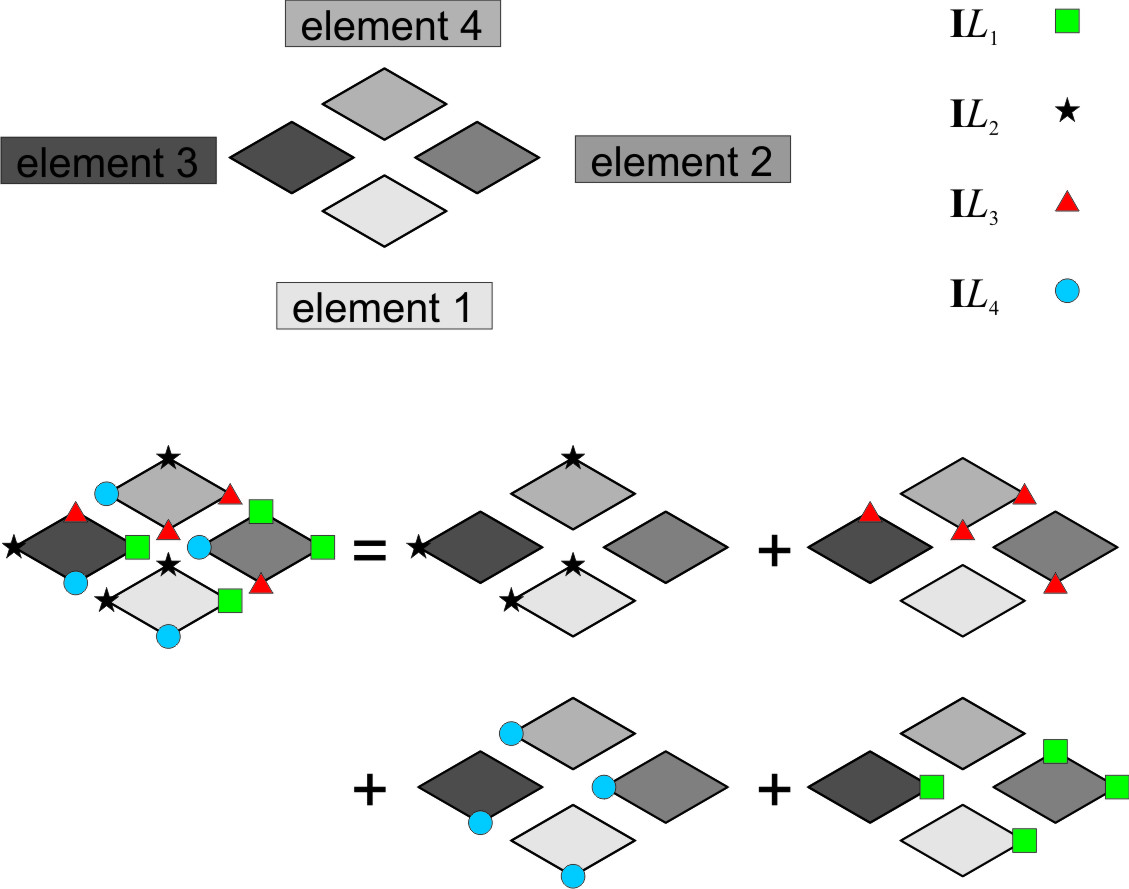
\includegraphics[width=0.8\textwidth]{beamer_figs/mesh_colouring_scheme4.jpg}	
			\label{fig:mesh_colouring}
	\end{figure}
\end{frame}
%%%%%%%%%%%%%%%%%%%%%%%%%%%%%%%%%%%%%%%%%%%%%%%%%%
\begin{frame}[t]{Delamination modelling}
	\begin{figure} [h!]
		\centering
		\includegraphics[width=\textwidth]{delam_modelling_shell.png}	
		\caption{The concept of delamination modelling: cross-section through the composite laminate and delamination showing three regions: (I) undelaminated, (II) above delamination interface, and (III) below delamination interface and corresponding elements.}
		\label{fig:delam_modelling_shell}
	\end{figure}
\end{frame}
%%%%%%%%%%%%%%%%%%%%%%%%%%%%%%%%%%%%%%%%%%%%%%%%%%
\begin{frame}{Computation speedup analysis}
	\begin{table}
		\renewcommand{\arraystretch}{1.3}
		\centering \small
		Computation run times depending on the number of degrees of freedom (NDOF) for the wave propagation duration 400~$\mu$s; GPU: Nvidia Tesla K20X; CPU: Intel Xeon X5660 2.8~GHz.
		
		\begin{tabular}{ccccccc} 
			%\hline
			\toprule	
			plate size [cm] & 30$\times$30  & 40$\times$40 & 50$\times$50 & 70$\times$70 & 90$\times$90 & 100$\times$100 \\
			NDOF $\cdot 10^6$ & 1.02  & 1.46 & 1.98 & 3.09 & 5.23 & 6.36 \\
			\midrule
			CPU time [h]& 4.03& 5.71 & 8.42 & 13.13 & 22.37 & 27.33\\
			\midrule
			GPU time [h]& 1.00& 1.19 & 1.26 & 1.50 & 2.00 & 2.28\\
			%\hline 
			\bottomrule 
		\end{tabular} 
		\label{tab:run_time}
	\end{table}
\end{frame}
\begin{frame}{Computation speedup analysis}
	\begin{figure} [h!]
		\centering
		\includegraphics{speedup.png}	
		\caption{Computation speedup; NDOF - number of degrees of freedom.}
		\label{fig:speedup}
	\end{figure}
	\begin{equation*}
	speedup = \frac{CPU_{time}}{GPU_{time}}
	\label{eq:speedup}
	\end{equation*}
\end{frame}
%%%%%%%%%%%%%%%%%%%%%%%%%%%%%%%%%%%%%%%%%%%%%%%%%%
\section{Experimental validation}
%%%%%%%%%%%%%%%%%%%%%%%%%%%%%%%%%%%%%%%%%%%%%%%%%%
\begin{frame}{Open Guided Waves}
	\begin{block}{\url{http://www.open-guided-waves.de}}
		Open Guided Waves is an extendable online platform where high--quality and well documented datasets for guided wave--based inspections are provided.
	\end{block}

	CFRP plates [45/0/-45/90/-45/0/45/90]\textsubscript{S}
	
	500 mm $\times$ 500 mm, thickness of 2 mm. 
	
	Piezoelectric transducers diameter 10 mm, thickness 0.2 mm.
	
	\begin{table}
		\renewcommand{\arraystretch}{1.3}
		\centering \small
		Material properties of unidirectional Hexply M21/34\%/UD134/T700/300; Units: GPa.
		
		\begin{tabular}{cccccc} 
			%\hline
			\toprule
			$Q_{11}$ & $Q_{12}$  & $Q_{22}$ & $Q_{44}$ & $Q_{55}$ & $Q_{66}$\\
			% \cmidrule(lr){1-3} \cmidrule(lr){4-6} \cmidrule(lr){7-7}
			%\hline
			\midrule
			130& 6.1& 11.2 & 3.0 & 4.2 & 4.2\\
			%\hline 
			\bottomrule 
		\end{tabular} 
		\label{tab:mat_prop}
	\end{table}
\end{frame}
%%%%%%%%%%%%%%%%%%%%%%%%%%%%%%%%%%%%%%%%%%%%%%%%%%
\begin{frame}{Open Guided Waves}

	\begin{table}
		\renewcommand{\arraystretch}{1.3}
		\centering \small
		Coordinates of analysed defects; Units: [m].
		
		\begin{tabular}{cccc} 
			%\hline
			\toprule
			\multicolumn{2}{c}{\textbf{Data set I} }	& \multicolumn{2}{c}{\textbf{Data set II} } \\
			\multicolumn{2}{c}{\textbf{(wavefield plate)} }	& \multicolumn{2}{c}{\textbf{(SHM plate)} } \\
			%\midrule
			\cmidrule(lr){1-2} \cmidrule(lr){3-4}
			x & y &  x &  y  \\
			% \cmidrule(lr){1-3} \cmidrule(lr){4-6} \cmidrule(lr){7-7}
			%\hline
			0.191 & 0.145 & 0.250  & 0.427 \\ 
			%\hline 
			\bottomrule 
		\end{tabular} 
		\label{tab:defect_coordinates}
	\end{table}		
\end{frame}
%%%%%%%%%%%%%%%%%%%%%%%%%%%%%%%%%%%%%%%%%%%%%%%%%%
\begin{frame}[b]{Meshing - GMSH quadrilateral elements}
	\begin{figure}
		\centering
		\includegraphics[width=0.7\textwidth]{delam_Jochen_signals_D5_a_5mm_b_5mm_angle_0added_mass.png}		
		\caption{red -- piezoelectric transducers; green -- defect location}
		\label{fig:quad_mesh}
	\end{figure}	
\end{frame}
%%%%%%%%%%%%%%%%%%%%%%%%%%%%%%%%%%%%%%%%%%%%%%%%%%
\begin{frame}[t]{Meshing - spectral element mesh close up}
	\begin{figure}
		\centering
		\includegraphics[width=0.7\textwidth]{delam_Jochen_signals_D5_a_5mm_b_5mm_angle_0added_mass_spec_zoom.png}	
		\label{fig:spec_mesh_zoom}
	\end{figure}	
\end{frame}
%%%%%%%%%%%%%%%%%%%%%%%%%%%%%%%%%%%%%%%%%%%%%%%%%%
\begin{frame}[t]{Wavefield plate: comparison of wavefields}
%\vspace{6pt}
\def\myindenta{0.01\textwidth} % define myindenta variable  for correcting caption placement
\begin{columns}[T]
	\column{0.5\textwidth}
		\begin{figure}
			\only<1>{
			\includegraphics[width=\textwidth]{exp_frame64.png}
			\caption{\hspace{\myindenta}Experimental wavefield at 112.5 $\mu$s}
			}
			\only<2>{
			\includegraphics[width=\textwidth]{exp_frame100.png}
			\caption{\hspace{\myindenta}Experimental wavefield at 168.7 $\mu$s}
			}
			\only<3>{
				\includegraphics[width=\textwidth]{exp_frame64.png}
				\caption{\hspace{\myindenta}Experimental wavefield at 112.5 $\mu$s}
			}
			\only<4>{
				\includegraphics[width=\textwidth]{exp_frame100.png}
				\caption{\hspace{\myindenta}Experimental wavefield at 168.7 $\mu$s}
			}
		\end{figure}
	\column{0.5\textwidth}
		\begin{figure}
			\only<1>{
			\includegraphics[width=\textwidth]{Vz_1_frame72_bottom.png}
			\caption{\hspace{\myindenta}Simulation (delamination) at 112.5 $\mu$s}
			}
			\only<2>{
			\includegraphics[width=\textwidth]{Vz_1_frame108_bottom.png}
			\caption{\hspace{\myindenta}Simulation (delamination) at 168.7 $\mu$s}
			}
			\only<3>{
				\includegraphics[width=\textwidth]{added_mass_Vz_1_frame72_bottom.png}
				\caption{\hspace{\myindenta}Simulation (added mass) at 112.5 $\mu$s}
			}
			\only<4>{
				\includegraphics[width=\textwidth]{added_mass_Vz_1_frame108_bottom.png}
				\caption{\hspace{\myindenta}Simulation (added mass) at 168.7 $\mu$s}
			}
			\label{fig:wavefield}
		\end{figure}
\end{columns}
	\only<5>{
	\begin{alertblock}{Remarks}
		Simulated wavefield patterns matches the experimental data very well.
	\end{alertblock}
	}
\end{frame}

%%%%%%%%%%%%%%%%%%%%%%%%%%%%%%%%%%%%%%%%%%%%%%%%%%
\begin{frame}[t]{SHM plate: comparison of signals}
	\begin{figure}
		\centering
		\only<1>{
		\includegraphics[width=0.9\textwidth]{path_1_7.png}	
		\label{fig:path1_7}
		}
		\only<2>{
			\includegraphics[width=0.9\textwidth]{path_2_4.png}	
			\label{fig:path2_4}
		}
		\only<3>{
			\includegraphics[width=0.9\textwidth]{path_4_8.png}	
			\label{fig:path4_8}
		}
		\only<4>{
			\includegraphics[width=0.9\textwidth]{path_2_4_diff.png}	
			\label{fig:path2_4_diff}
		}
	\end{figure}
	\only<5>{
		\begin{alertblock}{Remarks}
			Differences between experimental and numerical signals are evident and are related to amplitude rather than wave velocity.
		\end{alertblock}
	}	
\end{frame}
%%%%%%%%%%%%%%%%%%%%%%%%%%%%%%%%%%%%%%%%%%%%%%%%%%
\begin{frame}{Blocks}
  Three different block environments are pre-defined and may be styled with an
  optional background color.

  \begin{columns}[T,onlytextwidth]
    \column{0.5\textwidth}
      \begin{block}{Default}
        Block content.
      \end{block}

      \begin{alertblock}{Alert}
        Block content.
      \end{alertblock}

      \begin{exampleblock}{Example}
        Block content.
      \end{exampleblock}

    \column{0.5\textwidth}

     % \metroset{block=fill}

      \begin{block}{Default}
        Block content.
      \end{block}

      \begin{alertblock}{Alert}
        Block content.
      \end{alertblock}

      \begin{exampleblock}{Example}
        Block content.
      \end{exampleblock}

  \end{columns}
\end{frame}
%%%%%%%%%%%%%%%%%%%%%%%%%%%%%%%%%%%%%%%%%%%%%%%%%%
\begin{frame}{Future works}
	\begin{figure}
		\centering
		\only<1>{
			\includegraphics[width=0.75\textwidth]{beamer_figs/RMS5.png}	
			\label{fig:random_exc_wavefield_RMS5}
		}
		\only<2>{
			\includegraphics[width=0.75\textwidth]{beamer_figs/RMS14.png}	
			\label{fig:random_exc_wavefield_RMS14}
		}
		\only<3>{
			\includegraphics[width=0.75\textwidth]{beamer_figs/RMS22.png}	
			\label{fig:random_exc_wavefield_RMS22}
		}
	\end{figure}	
\end{frame}

%%%%%%%%%%%%%%%%%%%%%%%%%%%%%%%%%%%%%%%%%%%%%%%%%%

%%%%%%%%%%%%%%%%%%%%%%%%%%%%%%%%%%%%%%%%%%%%%%%%%%

%%%%%%%%%%%%%%%%%%%%%%%%%%%%%%%%%%%%%%%%%%%%%%%%%%
\section{Conclusion}
%%%%%%%%%%%%%%%%%%%%%%%%%%%%%%%%%%%%%%%%%%%%%%%%%%
\begin{frame}{Summary}

  Get the source of this theme and the demo presentation from

  \begin{center}\url{github.com/matze/mtheme}\end{center}

  The theme \emph{itself} is licensed under a
  \href{http://creativecommons.org/licenses/by-sa/4.0/}{Creative Commons
  Attribution-ShareAlike 4.0 International License}.

  \begin{center}\ccbysa\end{center}

\end{frame}
%%%%%%%%%%%%%%%%%%%%%%%%%%%%%%%%%%%%%%%%%%%%%%%%%%
{\setbeamercolor{palette primary}{fg=black, bg=white}
\begin{frame}[standout]
  Thank you for your attention!\\ \vspace{12pt}
  Questions?\\ \vspace{12pt}
  \url{pk@imp.gda.pl}
\end{frame}
}
%%%%%%%%%%%%%%%%%%%%%%%%%%%%%%%%%%%%%%%%%%%%%%%%%%
% END OF SLIDES
%%%%%%%%%%%%%%%%%%%%%%%%%%%%%%%%%%%%%%%%%%%%%%%%%%
\appendix
%%%%%%%%%%%%%%%%%%%%%%%%%%%%%%%%%%%%%%%%%%%%%%%%%%
\begin{frame}{Backup slides}
  \begin{equation*}
  \begin{split}
  \bs{\sigma}_{xx}&=\left((\bm{N},_{\xi}\vec{U}_x).*(\vec{J}^{-1})_{11}+(\bm{N},_{\eta}\vec{U}_x).*(\vec{J}^{-1})_{21}\right).*\vec{A}_{11}\\
  &+\left((\bm{N},_{\xi}\bs{\Phi}_x).*(\vec{J}^{-1})_{11}+(\bm{N},_{\eta}\bs{\Phi}_x).*(\vec{J}^{-1})_{21}\right).*\vec{B}_{11}\\
  &+\left((\bm{N},_{\xi}\vec{U}_y).*(\vec{J}^{-1})_{12}+(\bm{N},_{\eta}\vec{U}_y).*(\vec{J}^{-1})_{22}\right).*\vec{A}_{12}\\
  &+\left((\bm{N},_{\xi}\bs{\Phi}_y).*(\vec{J}^{-1})_{12}+(\bm{N},_{\eta}\bs{\Phi}_y).*(\vec{J}^{-1})_{22}\right).*\vec{B}_{12}\\
  &+\left((\bm{N},_{\xi}\vec{U}_x).*(\vec{J}^{-1})_{12}+(\bm{N},_{\eta}\vec{U}_x).*(\vec{J}^{-1})_{22}\right).*\vec{A}_{16}\\
  &+\left((\bm{N},_{\xi}\bs{\Phi}_x).*(\vec{J}^{-1})_{12}+(\bm{N},_{\eta}\bs{\Phi}_x).*(\vec{J}^{-1})_{22}\right).*\vec{B}_{16}\\
  &+\left((\bm{N},_{\xi}\vec{U}_y).*(\vec{J}^{-1})_{11}+(\bm{N},_{\eta}\vec{U}_y).*(\vec{J}^{-1})_{21}\right).*\vec{A}_{16}\\
  &+\left((\bm{N},_{\xi}\bs{\Phi}_y).*(\vec{J}^{-1})_{11}+(\bm{N},_{\eta}\bs{\Phi}_y).*(\vec{J}^{-1})_{21}\right).*\vec{B}_{16},
  \end{split}
  \end{equation*}
  where $.*$ denotes element-wise operation known as Hadamarad product (the same symbol for element-wise operation is used in Matlab). It should be noted that $\vec{A}$, $\vec{B}$, $\vec{D}$ and $(\vec{J}^{-1})$ with appropriate indexes are arranged in the form of vectors respective to GLL nodes of consecutive disjoint spectral elements.
\end{frame}
%%%%%%%%%%%%%%%%%%%%%%%%%%%%%%%%%%%%%%%%%%%%%%%%%%
\begin{frame}{Backup slides}
	\begin{equation*}
	\vec{U}_x = \left[
	\begin{array}{c}  
	\hat{\vec{u}}_0^{e=1}  \\[2pt]
	\hat{\vec{u}}_0^{e=2} \\[2pt]
	\vdots\\[2pt]
	\hat{\vec{u}}_0^{e=n}\\[2pt]
	\end{array}\right],
	\quad
	\vec{U}_y = \left[
	\begin{array}{c}  
	\hat{\vec{v}}_0^{e=1}  \\[2pt]
	\hat{\vec{v}}_0^{e=2} \\[2pt]
	\vdots\\[2pt]
	\hat{\vec{v}}_0^{e=n}\\[2pt]
	\end{array}\right],
	\quad
	\vec{U}_z = \left[
	\begin{array}{c}  
	\hat{\vec{w}}_0^{e=1}  \\[2pt]
	\hat{\vec{w}}_0^{e=2} \\[2pt]
	\vdots\\[2pt]
	\hat{\vec{w}}_0^{e=n}\\[2pt]
	\end{array}\right],
	\end{equation*}
	\begin{equation*}
	\bs{\Phi}_x = \left[
	\begin{array}{c}  
	\hat{\bs{\varphi}}_x^{e=1}  \\[2pt]
	\hat{\bs{\varphi}}_x^{e=2} \\[2pt]
	\vdots\\[2pt]
	\hat{\bs{\varphi}}_x^{e=n}\\[2pt]
	\end{array}\right],
	\quad
	\bs{\Phi}_y = \left[
	\begin{array}{c}  
	\hat{\bs{\varphi}}_y^{e=1}  \\[2pt]
	\hat{\bs{\varphi}}_y^{e=2} \\[2pt]
	\vdots\\[2pt]
	\hat{\bs{\varphi}}_y^{e=n}\\[2pt]
	\end{array}\right],
	\end{equation*}
	$n$ is the total number of elements.\\	
\end{frame}	
%%%%%%%%%%%%%%%%%%%%%%%%%%%%%%%%%%%%%%%%%%%%%%%%%%
\begin{frame}{Backup slides}
	Sparse matrices of shape function derivatives:
	\begin{equation*}
	\bm{N},_{\xi} = \left[
	\begin{array}{cccc}  
	\bm{N},_{\xi}^{e=1} & 0 & \ldots & 0\\[2pt]
	0& \bm{N},_{\xi}^{e=2}  & \ldots& 0\\[2pt]
	\vdots&\vdots&\ddots&0\\[2pt]
	0& 0 &0&\bm{N},_{\xi}^{e=n}\\[2pt]
	\end{array}\right].
	\end{equation*}
\end{frame}
%%%%%%%%%%%%%%%%%%%%%%%%%%%%%%%%%%%%%%%%%%%%%%%%%%
\begin{frame}{Backup slides}
\begin{equation*}
\begin{split}
\vec{F}_u^i&=\bm{N},_{\xi}^T \left(\bs{\sigma}_{xx}\,.*(\vec{J}^{-1})_{11}\,.*\vec{W}\right)+\bm{N},_{\eta}^T \left(\bs{\sigma}_{xx}\,.*(\vec{J}^{-1})_{21}\,.*\vec{W}\right)\\
&+\bm{N},_{\xi}^T \left(\bs{\sigma}_{xy}\,.*(\vec{J}^{-1})_{12}\,.*\vec{W}\right)+\bm{N},_{\eta}^T \left(\bs{\sigma}_{xy}\,.*(\vec{J}^{-1})_{22}\,.*\vec{W}\right), \\ 
\vec{F}_v^i&=\ldots ,\\
\vec{F}_w^i&=\ldots ,\\
\vec{M}_x^i&=\bm{N},_{\xi}^T \left(\bs{\sigma}_{xxz}\,.*(\vec{J}^{-1})_{11}\,.*\vec{W}\right)+\bm{N},_{\eta}^T \left(\bs{\sigma}_{xxz}\,.*(\vec{J}^{-1})_{21}\,.*\vec{W}\right)\\
&+\bm{N},_{\xi}^T \left(\bs{\sigma}_{xyz}\,.*(\vec{J}^{-1})_{12}\,.*\vec{W}\right)+\bm{N},_{\eta}^T \left(\bs{\sigma}_{xyz}\,.*(\vec{J}^{-1})_{22}\,.*\vec{W}\right)\\
&+\bs{\sigma}_{xz}\,.*\vec{W},\\
\vec{M}_y^i&=\ldots ,
\label{eq:internal_forces}
\end{split}
\end{equation*}
where $^T$ is the matrix transpose and $\vec{W}$ is the vector resulting from multiplication of integration weights and Jacobian determinant at appropriate GLL points:
\begin{equation*}
\vec{W} = \vec{w}_{\xi}\,.*\vec{w}_{\eta}\,.*\left(\det\vec{J}\right).
\end{equation*}
\end{frame}
\end{document}